\chapter{Fuzzy Clustering}
\label{chapter:fuzzy}

En este capítulo estaremos utilizando \gls{FCM} para encontrar clusters en nuestros conjuntos de datos, usando en particular la implementación proveída por la librería \textit{scikit-fuzzy} en Python \citep{2020SciPy-NMeth}.

\gls{FCM} es un método de clustering en el cual cada punto de los datos puede pertenecer a más de un cluster, mediante la asignación de valores de pertenencia a cada punto de nuestros datos por cada cluster que estemos buscando. Así, puntos cerca del borde de un cluster obtienen un bajo valor de pertenencia.

Formalmente, dado un conjunto de datos $X = (x_1, x_2,..., x_k)$, si tenemos en total $k$ puntos de datos y $c$ clusters, entonces se define la función de pertenencia como:

\begin{equation}
    \begin{aligned}
        \mu_{ij} = \mu_i(x_j) \in [0, 1] \ \ \forall i = 1,...,c \land \forall j = 1,...,k
    \end{aligned}
\end{equation} 

De forma tal que

\begin{equation}
    \begin{aligned}
        \sum_{i=1}^{c} \mu_i(x_j) = 1 \ \ \forall j = 1,...,k.
    \end{aligned}
\end{equation} 

Se define a una partición difusa como la caracterización de la participación de cada muestra en todos los clusters a partir de un valor de pertenencia que se encuentra en el rango $[0, 1]$. Estas particiones difusas se representan con una matriz, asociando cada fila a uno de los $c$ clusters y cada columna a uno de los elementos de $X$, de forma tal que el valor en la fila $i$ y la columna $j$ indique la pertenencia del elemento $j$ al cluster $i$. Puede definirse el conjunto de particiones difusas de la siguiente manera:

\begin{equation}
    \begin{aligned}
        M_{fc} = \{U \in \Re^{c \times n} | U = [u_{ij}];u_{ij} \in [0, 1] \forall i, j; \sum_{i=1}^{c} u_{ij} = 1  \forall j; \sum_{j=1}^{k} u_{ij} > 0  \forall i \}
    \end{aligned}
\end{equation}

Por lo tanto, podemos traducir el problema de \gls{FCM} a buscar una partición difusa (es decir, una matriz perteneciente al conjunto descrito arriba) óptima.

El algoritmo que utilizaremos para converger en una matriz pertenece al grupo de Fuzzy c-Means, los cuales a su vez forman parte de una clase de algoritmos basados en funciones objetivo. Por lo cual, pasaremos a definir la siguiente función de error mínimo cuadrático la cual el algoritmo minimizara de forma iterativa, para así encontrar la partición difusa óptima:

\begin{equation}
    \begin{aligned}
        J_m(U, v) = \sum_{j=1}^{k} \sum_{i=1}^{c} (u_{ij})^m d_{ij}^2
    \end{aligned}
\end{equation} 

En donde $d_{ij}$ es la distancia Euclidiana entre el elemento $x_j$ y el centro del cluster $i$, mientras que $U \in M_{fc}$ contiene todos los pesos $u_{ij}$ asociados a las distancias cuadradas y $v$ representa el vector centro de cada cluster. El valor de $m$ representa qué tan difusa queremos que sea la partición, con valores  $m \rightarrow 1$ dando como resultado valores de pertenencia más distintivos (obteniendo resultados similares a k-means), mientras que con $m \rightarrow \infty$ la partición óptima se aproximará a la matriz en donde todos sus valores son $1/c$.

Una vez definida la función objetivo, el algoritmo se basa en seguir los siguientes pasos:
\begin{enumerate}
  \item Fijar $c$, $k$ y $m$. Elegir una matriz inicial $U^{(0)}\in M_{fc}$
  \item Calcular los centros de los clusters como $v_{i}={\frac {\sum \limits _{j=1}^{k}(u_{ij})^{m}x_{j}}{\sum \limits _{j=1}^{k}(u_{ij})^{m}}};1\leq i\leq c$
  \item Actualizar la matriz de partición difusa $U = [uij]$ con $u_{ij}=(\sum \limits _{n=1}^{c}({\frac {d_{ij}}{d_{nj}}})^{\frac {2}{m-1}})^{-1};1\leq j\leq k;1\leq i\leq c$
  \item Si se alcanzó la máxima cantidad de iteraciones, o la diferencia de la matriz U con respecto a la iteración anterior es menor al error mínimo dado, el algoritmo termina. Caso contrario, vuelve al paso 2.
\end{enumerate}

Una vez terminado de correr el algoritmo, etiquetamos cada dato de nuestro conjunto con el cluster cuyo valor en la partición difusa sea mayor.

\section{Detección de dos componentes: Disco y esferoide}

Antes de comenzar es necesario entender que utilizar algoritmos de clasificación con una sola feature del dataset no podrá introducir un limite ``difuso'' entre clusters, ya que los números no tendrán ningún significado para el método, a diferencia de Abadi que les da una interpretación física. Por lo cual, si pedimos al algoritmo que busque clusters en una recta, no va a tener otras dimensiones de las cuales extraer información para entender donde los clusters se pueden solapar, haciendo que éstos siempre tengan una separación clara entre ellos, sin importar el valor de fuzziness utilizado. Esto implica que al mejor resultado que se puede aspirar al comparar este método con Abadi es un corte vertical sobre $eps$ entre ambos clusters que se encuentra lo más cercano posible al valor donde la densidad del Disco pasa a ser menor que la del Esferoide en los obtenidos con Abadi.

Curiosamente, mientras buscábamos hiperparámetros, notamos que el valor de ``corte'' en $eps$ que separa las dos clases encontradas se mueve hacia la derecha en la recta al aumentar el valor de fuzziness, como mostramos en la Fig ~\ref{fig:FC2componentesHistFuzzinesComparison}.

\begin{figure}
    \centering
    
\includegraphics[width=9cm]{fuzzy clustering/figures/galaxy_TNG_375401 - Abadi - circ histogram fuzzines comparison.png}
    \caption{Histograma comparando los resultados obtenidos con \gls{FCM} con diferentes valores de fuzziness sobre la galaxia \textit{galaxy\_TNG\_375401} en espacio circular.}
    \label{fig:FC2componentesHistFuzzinesComparison}
\end{figure}


Si observamos la ecuación del segundo paso del algoritmo descrito en la sección anterior, podemos observar cómo aumentar el valor de fuzziness implica que el peso que tendrán los valores de pertenencia en la ecuación disminuirá, reduciendo las diferencias entre ellos. Esto asigna similar relevancia a cada punto para cada cluster, haciendo que éstos sean más ``heterogéneos'', pero este efecto no es justificación suficiente para explicar el comportamiento visto al aumentar el valor de fuzziness.

Al investigar el código de la librería usada para aplicar este método nos encontramos con que los valores de pertenencia de cada punto son representados por \texttt{float64}, cuyo mínimo valor representable es $2.2250738585072014 \times 10^{-308}$. Esto no parece ser un problema a simple vista, ya que los valores de pertenencia suelen ser mayores, pero si nos detenemos por ejemplo en el primer cuartil de los valores de pertenencia del Esferoide para la galaxia $TNG\_375401$ vemos que éste es $7.56 \times 10^{-5}$. Con este valor, basta un valor de fuzziness de 75 para superar el mínimo valor representable por $float64$ en el segundo paso del algoritmo descrito, volviendo los pesos de un cuarto de los puntos del dataset nulos para el centro del Disco.

Por lo tanto, el peso que tendrán los puntos más alejados de cada cluster será nulos para el segundo paso del algoritmo, lo que provoca que las partículas que se encuentran más cercanas al extremo izquierdo de la recta no afectarán al cálculo del centro del cluster del Esferoide. Como la cantidad de partículas pertenecientes a dicha componente cuyo peso dejará de afectar al cálculo del centro del cluster se encuentran mayoritariamente en el extremo izquierdo del cluster (ya que el extremo derecho está cerca del centro, por lo cual sus valores de pertenencias siguen siendo relevantes), entonces se moverá el centro de la componente hacia la derecha, como se muestra en la Tabla~\ref{table:2componentesFC375401}.

\begin{table}[h!]
\centering
\begin{tabular}{|c|c|c|}
\hline
Fuzziness&Centro de Esferoide&Centro de Disco\\
\hline
$1.4$ & $-0.078$ & $0.616$\\
\hline
$14$ & $0.008$ & $0.647$\\
\hline
$140$ & $0.027$ & $0.643$\\
\hline
\end{tabular}
\caption{Centros de los clusters encontrados por \gls{FCM} en $eps$ sobre la galaxia \textit{galaxy\_TNG\_375401} al aumentar el valor de fuzziness.}
\label{table:2componentesFC375401}
\end{table}

Sucede un efecto similar en el Disco. Las partículas de éste que se encuentren más a la izquierda en la recta pasaran a tener peso nulo en el cálculo de su centro, derivando en el desplazamiento a la derecha de éste (aunque en menor medida).

Ambas razones resultan en que partículas que se encuentren entre el centro del Esferoide y el Disco en la recta y las cuales antes tenían un valor de pertenencia al Disco mayor que el valor de pertenencia al Esferoide, pasen a formar parte del Esferoide, moviendo la línea de corte hacia la derecha en el proceso. Por lo tanto, entre más grande es el valor de fuzziness, la diferencia entre los puntos que pasaran a no formar parte del cálculo de centros de clusters entre el Esferoide y el Disco se incrementará aún más, moviendo el corte hacia la derecha en la misma medida. Una vez entendido eso, dado el dominio de resultados posibles, pasamos a elegir un valor de fuzziness que acerque la línea de corte al punto promedio en donde la densidad del Disco supera a la del Esferoide en todas las galaxias de nuestro dataset. Luego de recorrer un amplio rango de valores de fuzziness, terminamos optando por $1.4$ como valor a utilizar para maximizar los valores de recall promedio de todas las galaxias, como podemos observar en Fig~\ref{fig:FC2componentesRecall}.

Además, en las pruebas que hicimos concluimos que fijar el error mínimo en $0.00005$ era suficiente para obtener buenos resultados, y disminuirlo aún más no resultaba en una gran diferencia en cantidad de iteraciones. Por su parte, fijamos la cantidad máxima de iteraciones en $1000$, aunque el algoritmo siempre terminó a partir de la condición de parada del error mínimo.

\begin{figure}
    \centering
    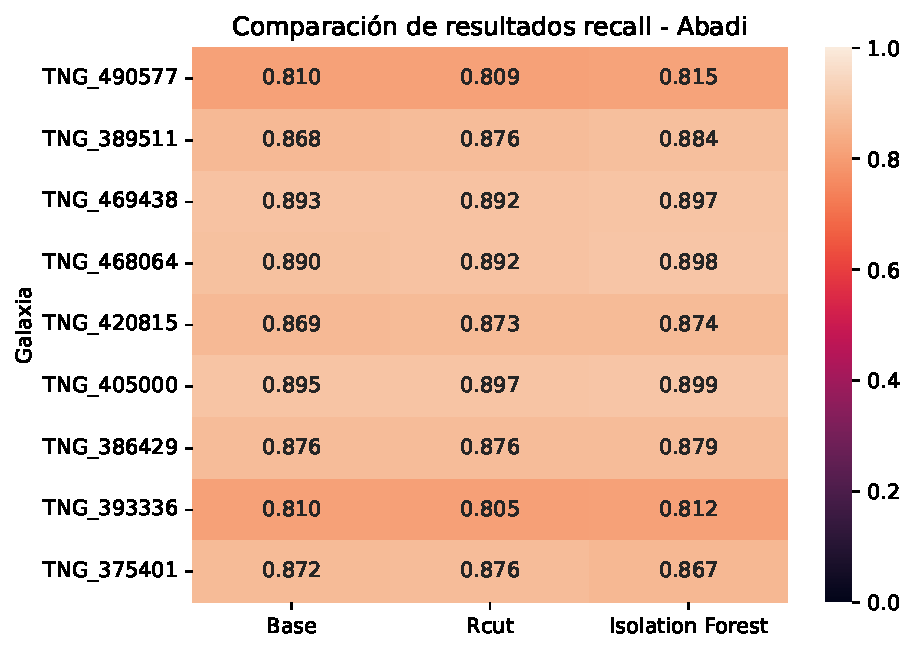
\includegraphics[width=12cm]{fuzzy clustering/figures/abadi - recall.pdf}
    \caption{Comparación de recall sobre los resultados obtenidos por \gls{FCM}, considerando a Abadi como ground truth}
    \label{fig:FC2componentesRecall}
\end{figure}

Sabiendo cual es el mejor resultado al cual podemos apuntar y como los valores de recall fueron tan positivos, consideramos el resultado del experimento como exitoso y a Fuzzy Clustering como una buena alternativa al algoritmo de Abadi, siempre y cuando se entiendan sus limitaciones.

\subsection{Eliminación de outliers}

Aplicamos métodos de eliminación de outliers con la intención de eliminar posibles partículas que no pertenezcan a la galaxia y así obtener mejores resultados a la hora de clusterizar. Sin embargo, nos encontramos que al aplicar \gls{IF} y \gls{RCUT} apenas si modifican los conjuntos encontrados de forma perceptible, como parece indicar la Fig~\ref{fig:FC2componentesRecall} y la Fig~\ref{fig:FC2componentesOutlierRemovalComparison}. Esto también es fácilmente visto en la Fig~\ref{fig:FC2componentesRotationCurve}.

\begin{figure}
    \centering
    
\includegraphics[width=12cm]{fuzzy clustering/figures/galaxy_TNG_375401 - Abadi - outlier removal comparison.png}
    \caption{Curva de rotación sobre los resultados obtenidos con Abadi y \gls{FCM} sobre la galaxia \textit{galaxy\_TNG\_375401}, utilizando diferentes métodos de eliminación de outliers.}
    \label{fig:FC2componentesOutlierRemovalComparison}
\end{figure}

\begin{figure}
    \centering
    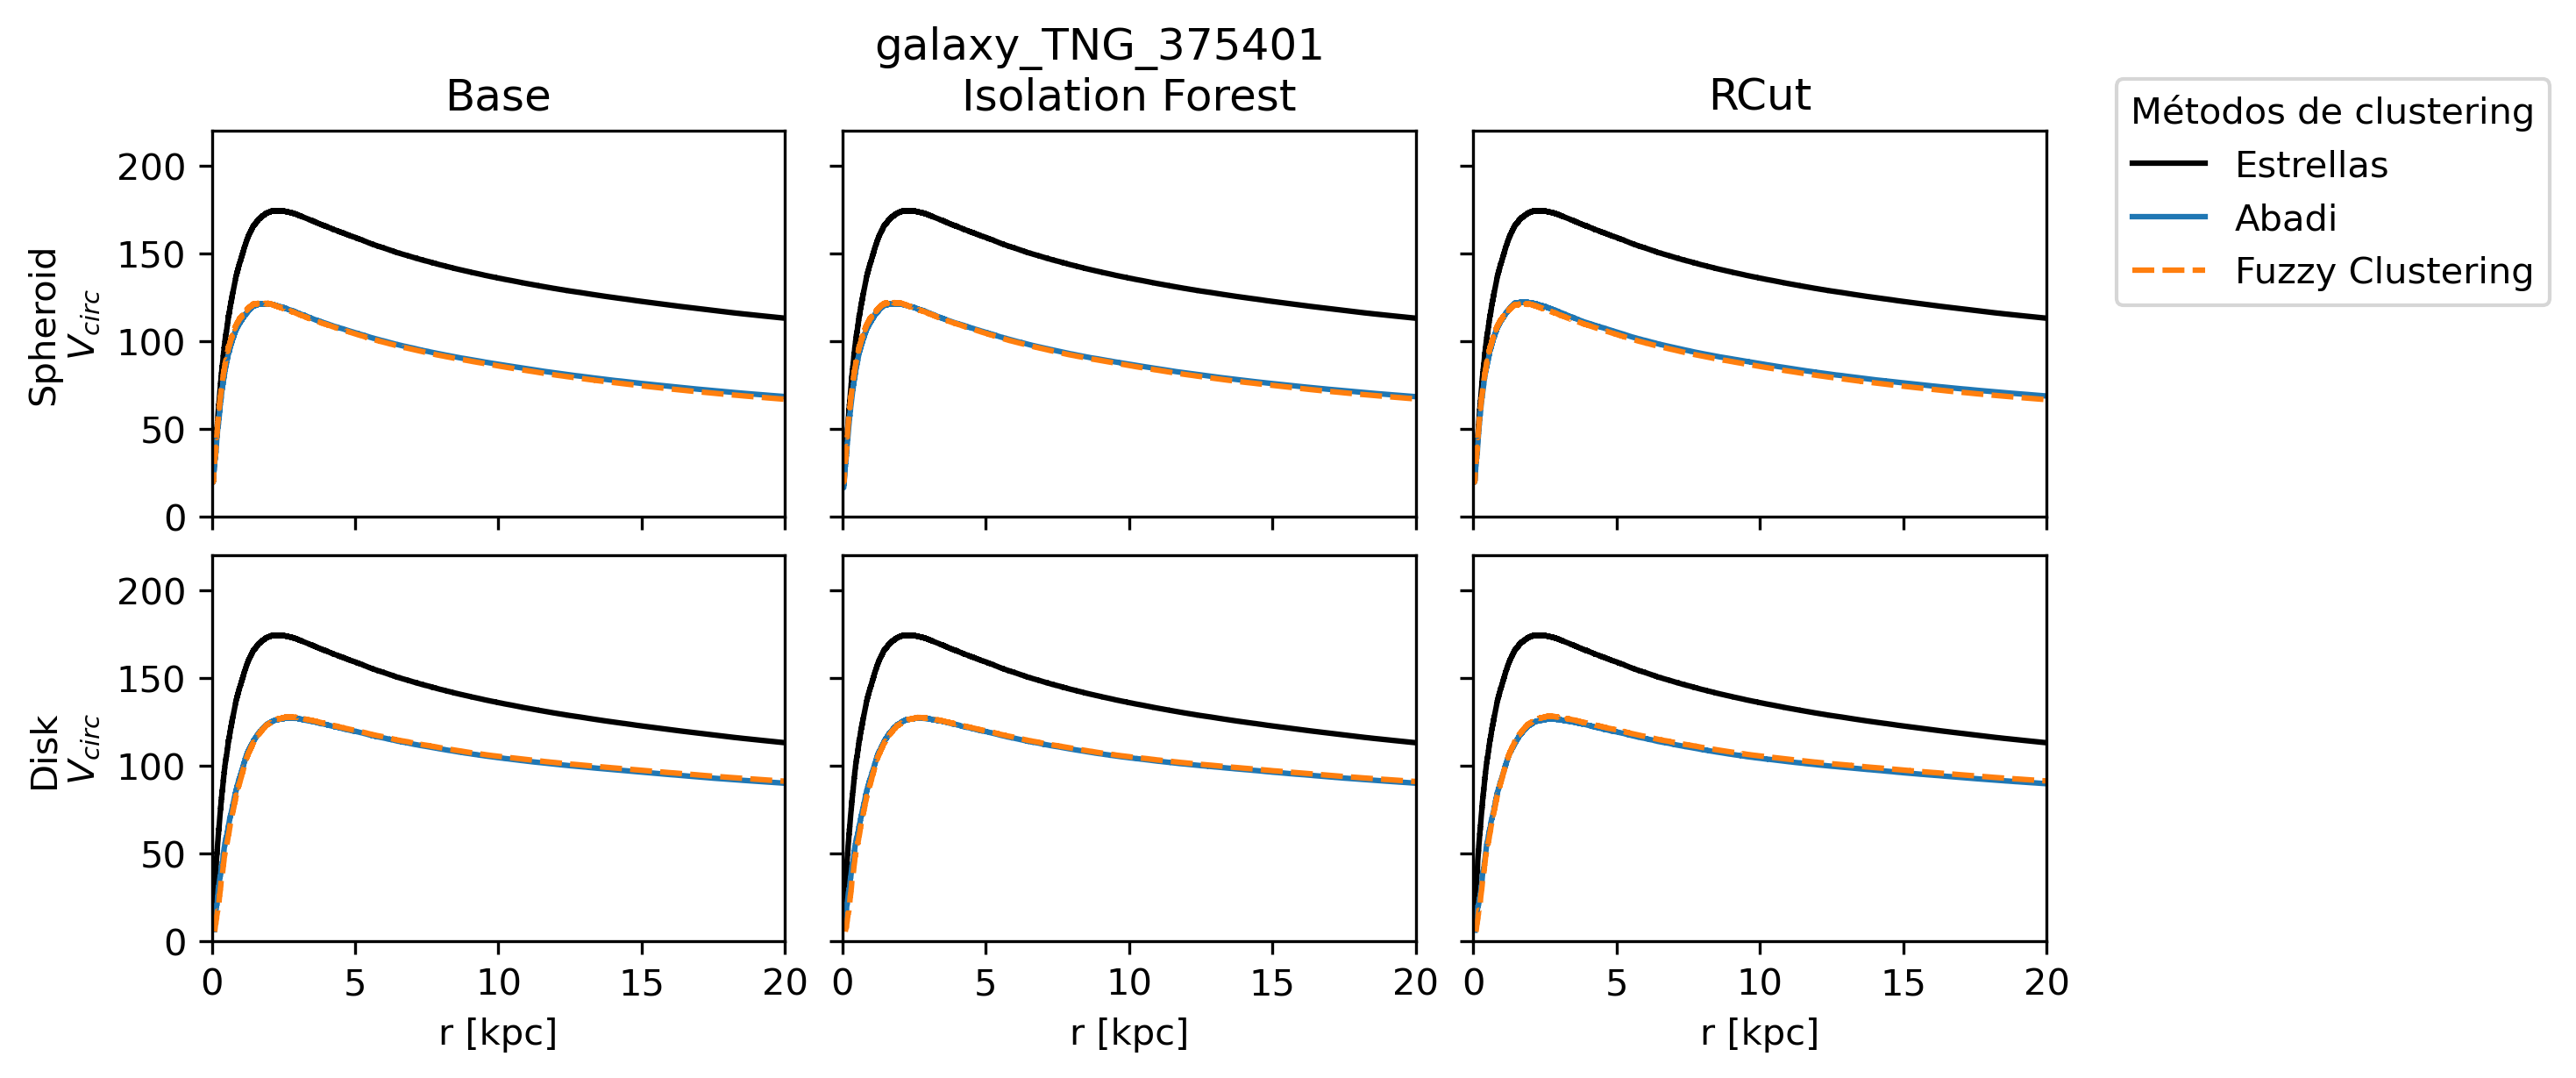
\includegraphics[width=12cm]{fuzzy clustering/figures/galaxy_TNG_375401 - Abadi - circ_velocity.png}
    \caption{Curva de rotación sobre los resultados obtenidos con Abadi y \gls{FCM} sobre la galaxia \textit{galaxy\_TNG\_375401}, utilizando diferentes métodos de eliminación de outliers.}
    \label{fig:FC2componentesRotationCurve}
\end{figure}

Esto se debe a que Fuzzy clustering es un método robusto dado que limita el impacto de los outliers al calcular los centros de los clusters \citep{580801}. Por esto, la presencia de outliers no modificará de forma significativa los clusters finales obtenidos, y en consecuencia, removerlos no llevará a conjuntos diferentes.

\section{Comparación con Auto Gaussian Mixture - $>$2 clusters}

Al igual que en la sección anterior, antes de comenzar con el experimento hicimos un análisis sobre los hiperparámetros para obtener el valor de fuzziness a utilizar. Pero a diferencia del análisis anterior, la búsqueda de dicho valor tuvo diferentes efectos sobre los resultados a partir de usar más de una feature a la hora de buscar clusters. Esto significa que la variación del valor de fuzziness tuvo el resultado esperado, y al variarlo y comparar los valores de recall obtenidos con los resultados provenientes de utilizar \gls{AGMM} concluimos que un valor de fuzziness de $3$ nos posiciona lo más cerca posible a los resultados obtenidos por este último.

Asimismo, mantendremos los valores de $0.00005$ y $1000$ utilizados para el mínimo error y la máxima cantidad de iteraciones que dispondrá el algoritmo, usados en la sección anterior.

Cuando comparamos \gls{HC} contra \gls{AGMM} en el capítulo anterior mencionamos como el clustering obtenido por el primero era prácticamente unidimensional siguiendo la feature de $eps$. Lamentablemente, los resultados vistos con \gls{FCM} son similares en este aspecto, como podemos observar en la Fig~\ref{fig:FCNcomponentesScatterplotTNG386429}.

\begin{figure}
    \centering
    
\includegraphics[width=12cm]{fuzzy clustering/figures/galaxy_TNG_386429 - circ scatterplot.png}
    \caption{Histograma comparando los resultados obtenidos con \gls{AGMM} contra los obtenidos con \gls{FCM} sobre la galaxia \textit{galaxy\_TNG\_386429} en espacio circular.}
    \label{fig:FCNcomponentesScatterplotTNG386429}
\end{figure}

Creemos que dicho resultado proviene de una ``sobre-relevancia'' de una feature sobre las otras. Si bien $eps$ es sin lugar a dudas la feature que mejor nos permite identificar clusters en nuestro conjunto de datos, $normalized\_star\_energy$ también contiene información importante, sobre todo para identificar el Halo y el Bulge, como puede observarse en el histograma de \gls{AGMM} en la Fig~\ref{fig:FCNcomponentesHistogramTNG386429}.

\begin{figure}
    \centering
    
\includegraphics[width=12cm]{fuzzy clustering/figures/galaxy_TNG_386429 - circ histogram.png}
    \caption{Histograma comparando los resultados obtenidos con \gls{AGMM} contra los obtenidos con \gls{FCM} sobre la galaxia \textit{galaxy\_TNG\_386429} en espacio circular.}
    \label{fig:FCNcomponentesHistogramTNG386429}
\end{figure}

Si nos detenemos sobre el tercer paso del algoritmo de \gls{FCM} podemos ver que éste deriva el valor de pertenencia de cada partícula con cada cluster a partir de la distancia de ésta hacia el centro de cada cluster. Sin embargo, observando las distribuciones de las partículas estelares en la Fig~\ref{fig:comparacion-features-circ-hist} podemos apreciar los rangos de valores que una partícula puede tener en cada feature; los valores de $eps$ tienen un rango $[-1, 1]$, mientras que el rango de los valores de $normalized\_star\_energy$ es $[-1, 0]$ y el de $eps\_r$ $[0, 1.5]$ (aunque a fines prácticos suele ser $[0, 1]$, incluso menor dependiendo la galaxia). Esto implica que, dada una partícula $x = (x.eps, x.normalized\_star\_energy, x.eps\_r)$ y un centro de cluster $c = (c.eps, c.normalized\_star\_energy, c.eps\_r)$, hay altas probabilidades de que la distancia de $x$ a $c$ sea mayormente dominada por la distancia entre $x.eps$ y $c.eps$.

\begin{figure}
    \centering
    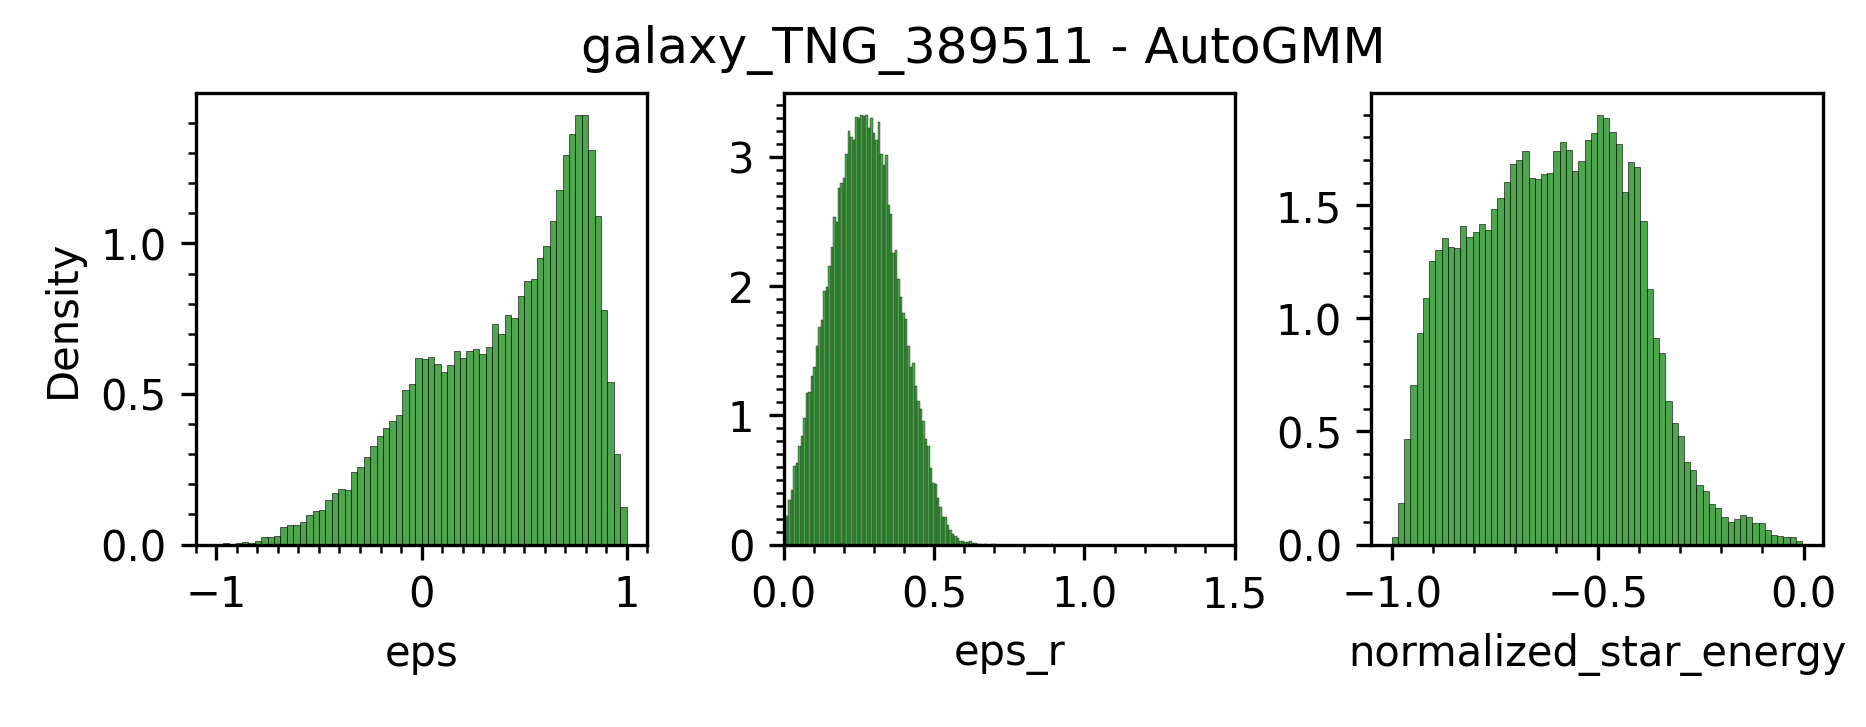
\includegraphics[width=12cm]{fuzzy clustering/figures/galaxy_TNG_389511 - circ histogram - features.png}
    \caption{Histograma comparando los rangos de valores en las cuales se acumulan las partículas estelares en cada feature del espacio circular de la galaxia \textit{galaxy\_TNG\_389511}.}
    \label{fig:comparacion-features-circ-hist}
\end{figure}

Curiosamente, podemos ver el efecto que tiene $normalized\_star\_energy$ sobre los valores de pertenencia al observar como en la Fig~\ref{fig:FCNcomponentesScatterplotTNG389511}, en $eps$ vs. $normalized\_star\_energy$ no tenemos líneas separadoras entre clusters totalmente rectas sino que son un tanto inclinadas. Dicha inclinación proviene del (leve) aporte que hace la feature de $normalized\_star\_energy$ sobre el valor de pertenencia de las partículas.

\begin{figure}
    \centering
    
\includegraphics[width=12cm]{fuzzy clustering/figures/galaxy_TNG_389511 - circ scatterplot.png}
    \caption{Histograma comparando los resultados obtenidos con \gls{AGMM} contra los obtenidos con \gls{FCM} sobre la galaxia \textit{galaxy\_TNG\_389511} en espacio circular.}
    \label{fig:FCNcomponentesScatterplotTNG389511}
\end{figure}

Se puede ver de forma aún más clara el poco impacto que tiene $normalized\_star\_energy$ en la clusterización realizada por \gls{FCM} en la Fig~\ref{fig:FCNcomponentesHistogramTNG389511}. En ella observamos como el Bulge y el Halo están solapados en $eps$ según el resultado obtenido por \gls{AGMM} (dado que el Esferoide está soportada por dispersión de velocidades, como se explicó en el capítulo anterior), pero son fácilmente distinguibles en $normalized\_star\_energy$. Además, se puede ver el nulo aporte de $eps\_r$ al clustering al observar los resultados de \gls{FCM} en el scatterplot de esta feature vs. $eps$ en la Fig~\ref{fig:FCNcomponentesScatterplotTNG389511} por lo rectas que son las delimitaciones entre las componentes encontradas.

\begin{figure}
    \centering
    
\includegraphics[width=12cm]{fuzzy clustering/figures/galaxy_TNG_389511 - circ histogram.png}
    \caption{Histograma comparando los resultados obtenidos con \gls{AGMM} contra los obtenidos con \gls{FCM} sobre la galaxia \textit{galaxy\_TNG\_389511} en espacio circular.}
    \label{fig:FCNcomponentesHistogramTNG389511}
\end{figure}

Vale la pena destacar que, aunque las componentes encontradas por \gls{FCM} difieran de los obtenidos por \gls{AGMM}, los centros de los clusters encontrados por el primero, mostrados en la Tabla~\ref{table:NcomponentesFC386429}, son bastante precisos y similares a lo observable con \gls{AGMM} en la Fig~\ref{fig:FCNcomponentesHistogramTNG386429}.

\begin{table}[h!]
\centering
\begin{tabular}{l|c|c|c|c|}
\cline{3-5}
\multicolumn{2}{c|}{}&center.eps&center.eps\_r&center.normalized\_star\_energy\\
\cline{2-5}
& Halo & $-0.066$ & $0.312$ & $-0.667$\\
\cline{2-5}
& Warm Disk & $0.632$ & $0.241$ & $-0.652$\\
\cline{2-5}
& Bulge & $0.320$ & $0.308$ & $-0.703$\\
\cline{2-5}
& Cold Disk & $0.831$ & $0.151$ & $-0.519$\\
\cline{2-5}
\end{tabular}
\caption{Features de los centros de los clusters encontrados por \gls{FCM} sobre la galaxia \textit{galaxy\_TNG\_386429}.}
\label{table:NcomponentesFC386429}
\end{table}

Algo que también notamos fue la rápida transición que realiza \gls{FCM} entre el Bulge y el Halo. La razón detrás de esto es similar a lo explicado sobre el rango total que cada feature puede cubrir. Si una partícula está a una distancia similar entre dos centros de clusters en cierta feature ($normalized\_star\_energy$ en este caso), entonces el peso que tendrán las distancias sobre esta feature a cada centro para calcular el valor de pertenencia de la partícula a cada cluster será similar entre ellas. Por esto las distancias en $eps$ serán las que definan los valores de pertenencia a cada componente sobre la feature mencionada, resultando de esta manera en el corte limpio entre ambas componentes. Dicho concepto es una continuación de lo visto en la sección anterior en la cual solo utilizamos $eps$ para clasificar.

Aunque esta idea está presente en todo nuestro dataset, se puede visualizar más claramente a partir de la Fig~\ref{fig:FCNcomponentesHistogramTNG393336} y la Tabla~\ref{table:NcomponentesFC393336}, y lo cerca que los centros de las componentes Bulge y Halo están entre ellos en $normalized\_star\_energy$.

\begin{figure}
    \centering
    
\includegraphics[width=12cm]{fuzzy clustering/figures/galaxy_TNG_393336 - circ histogram.png}
    \caption{Histograma comparando los resultados obtenidos con \gls{AGMM} contra los obtenidos con \gls{FCM} sobre la galaxia \textit{galaxy\_TNG\_393336} en espacio circular.}
    \label{fig:FCNcomponentesHistogramTNG393336}
\end{figure}

\begin{table}[h!]
\centering
\begin{tabular}{l|c|c|c|c|}
\cline{3-5}
\multicolumn{2}{c|}{}&center.eps&center.eps\_r&center.normalized\_star\_energy\\
\cline{2-5}
& Bulge & $0.005$ & $0.229$ & $-0.764$\\
\cline{2-5}
& Halo & $0.368$ & $0.197$ & $-0.713$\\
\cline{2-5}
& Warm Disk & $0.632$ & $0.206$ & $-0.586$\\
\cline{2-5}
& Cold Disk & $0.857$ & $0.145$ & $-0.399$\\
\cline{2-5}
\end{tabular}
\caption{Features de los centros de los clusters encontrados por \gls{FCM} sobre la galaxia \textit{galaxy\_TNG\_393336}.}
\label{table:NcomponentesFC393336}
\end{table}

Además, al observar el histograma en $eps$ en Fig~\ref{fig:FCNcomponentesHistogramTNG393336} también descubrimos una leve tendencia de \gls{FCM} a sobreestimar el Cold Disk (Disco Fino) por sobre el Warm Disk (Disco Grueso) con respecto a \gls{AGMM}.

Como el caso descrito previamente, la transición entre el Warm Disk y el Cold Disk encontrada por \gls{FCM} que podemos observar en dicho histograma tiene su origen en qué tan separados están los centros de ambas componentes en las features restantes, $normalized\_star\_energy$ y $eps_r$ (aunque el aporte de esta última a la clasificación sea mínimo, como se explicó arriba). Dado que la distancia entre ambas componentes es significativa en $normalized\_star\_energy$, como se puede ver en la Tabla~\ref{table:NcomponentesFC393336} (y a raíz del valor de fuzziness utilizado), existirá un solapamiento entre ambos clusters en el histograma de $eps$ en la Fig~\ref{fig:FCNcomponentesHistogramTNG393336}.

Podemos separar dicho solapamiento en dos zonas. La primera es la que se encuentra del Warm Disk yendo hacia el Cold Disk, y la segunda la que proviene de Cold Disk hacia el Warm Disk. Si comparamos la primera con la clusterización obtenida por \gls{AGMM} en el mismo sector, dado que la transición entre ambos es menos difusa, entonces habrá una sobre estimación del Cold Disk sobre el Warm Disk en este sector. En la segunda zona, aunque \gls{AGMM} también tenga una transición fuzzy, la densidad de Warm Disk es mayor a la que encuentra \gls{FCM}, obteniendo como resultado nuevamente una sobre estimación del Cold Disk sobre el Warm Disk. Dicho comportamiento puede ser visto en la mayoría de las galaxias de nuestro dataset en las cuales encontramos estas componentes.



\subsection{Eliminación de outliers}

Al igual que en el capítulo anterior, eliminar outliers antes de generar clusters con \gls{AGMM} puede resultar en un diferente grupo de componentes encontradas. Por esto reduciremos nuestro análisis a los casos en los cuales dicho conjunto de componentes se mantenía constante.

Sin embargo, como explicamos en la sección al comparar con Abadi, dada la robustez de \gls{FCM}, tampoco obtuvimos diferencia al remover outliers con \gls{RCUT} o \gls{IF} como puede observarse en la Fig~\ref{fig:FCNcomponentesCircVelocityTNG389511}.

\begin{figure}
    \centering
    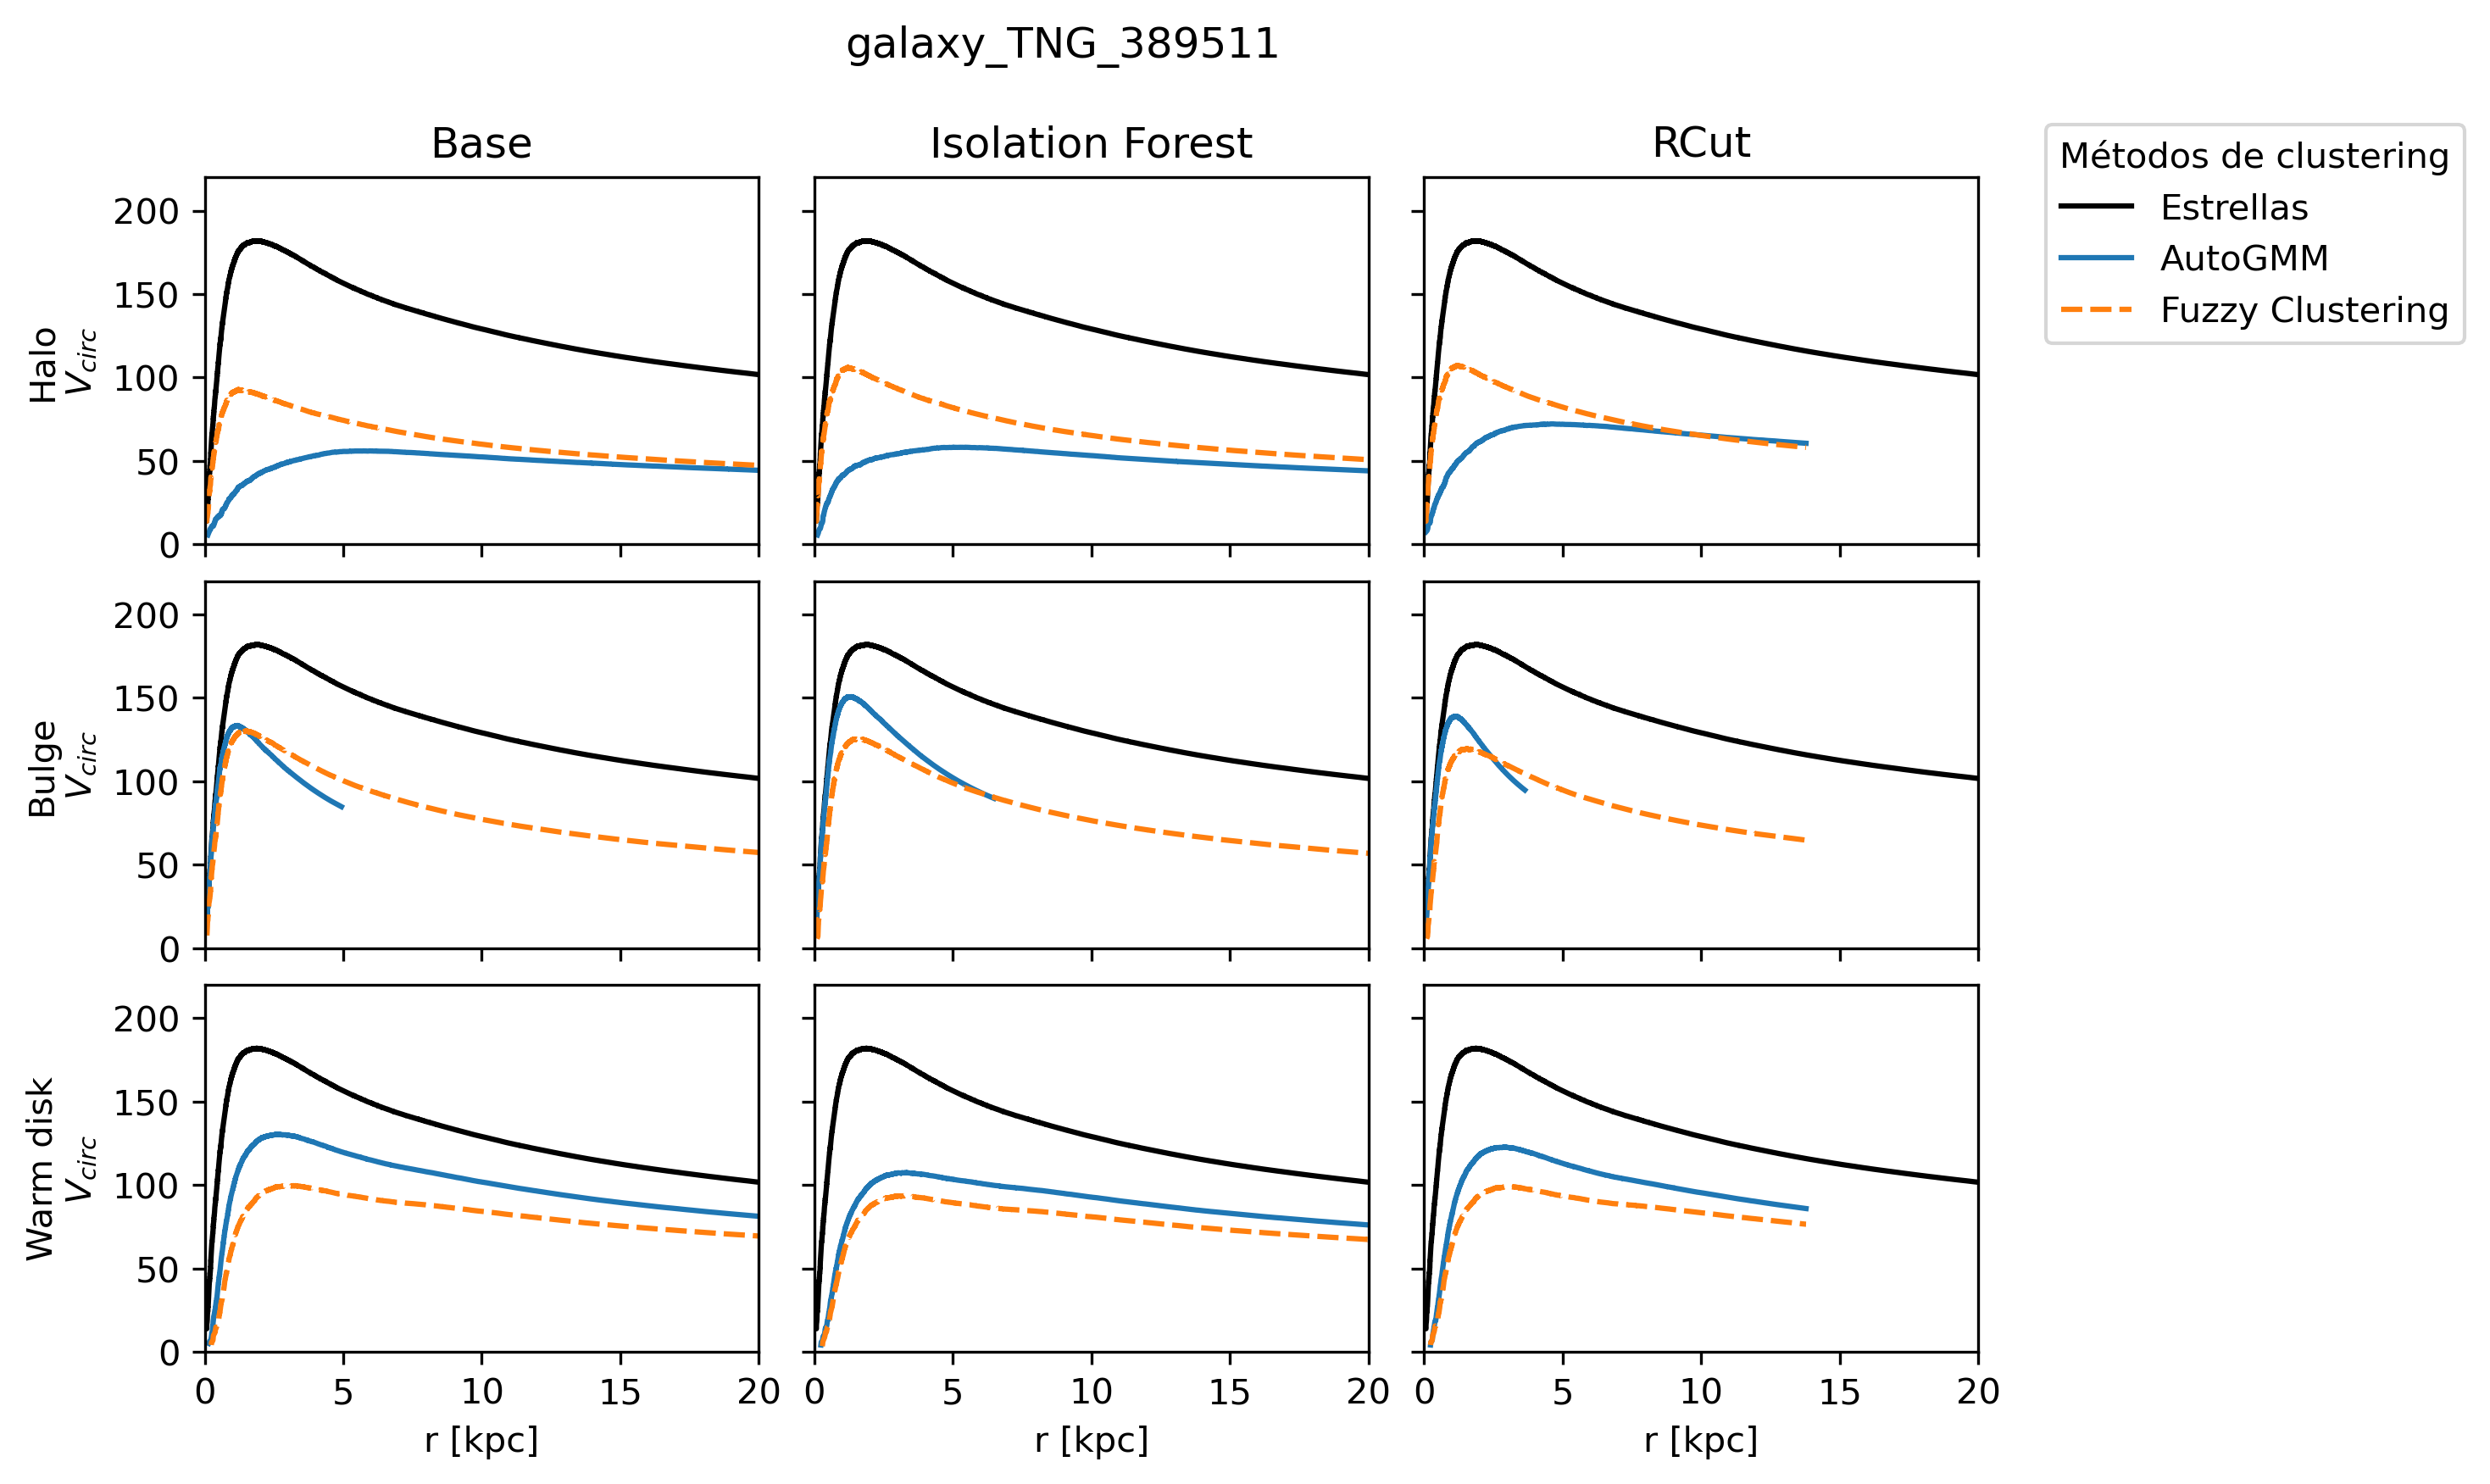
\includegraphics[width=12cm]{fuzzy clustering/figures/galaxy_TNG_389511 - AutoGMM - circ_velocity.png}
    \caption{Curva de rotación sobre los resultados obtenidos con \gls{AGMM} y \gls{FCM} sobre la galaxia \textit{galaxy\_TNG\_389511}, utilizando diferentes métodos de eliminación de outliers.}
    \label{fig:FCNcomponentesCircVelocityTNG389511}
\end{figure}

Para terminar, dado los resultados sub óptimos de las métricas de recall y precision (en promedio 0.626 y 0.698 respectivamente en nuestro dataset) concluimos que el método no es una buena alternativa a \gls{AGMM} al buscar más de dos componentes.

Sin embargo, dados los problemas explicados en esta sección, sería interesante en un trabajo futuro realizar una normalización sobre $eps$ y $eps_r$ previo a la clusterizacion de \gls{FCM} para promediar el peso que cada feature tiene sobre el conjunto de clusters finales.
